\documentclass[Main]{subfiles}

\begin{document}


\section{Designprocess}



\subsection{Fjernbetjening}

Projektet skulle indeholde en sender som kunne sende kommandoer til dronen.

\begin{figure}[H]
\centering
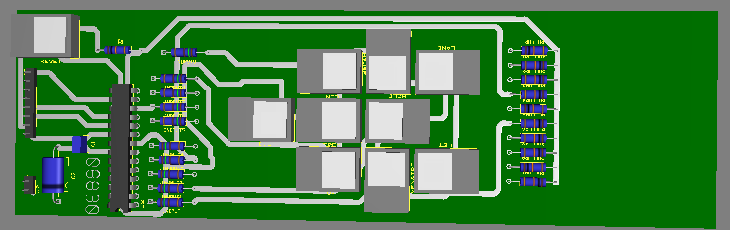
\includegraphics[width = 1 \textwidth]{3dUdenTal}
\caption{3D Figur af sender}
\label{Fig:3dUdenTal}
\end{figure}


Senderen som ses på figur \ref{Fig:3dUdenTal}, er bygget op i form som en fjernbetjening for, at det er muligt at betjene den med én hånd.
Fjernbetjeningen indeholder en µ-kontroller, radiosender og knapper.
Knapperne er her brugeren vælger et program/kommando der skal sendes til dronen. Når en knap bliver trykket ned, registrere µ-kontrolleren det. Denne genere så en frame med brugervalget. Denne frame bliver så sendt til radioen via SPI, hvorefter radioen får besked om at sende framen fra µ-kontrolleren.

\subsection{4+1 View}


\subsubsection*{Logic View}


\subsubsection*{Deployment View}


\subsubsection*{Process View}


\subsubsection*{Implementation View}

Koden til dronen, radiosenderen og radiomodtageren er skrevet i programmeringssproget C.

Der er tre projekter at arbejde videre på:

\begin{itemize}
\item Sender
\item Modtager
\item Drone
\end{itemize}

Det er muligt at videreudvikle på projektet.
En udførlig guide til hvordan man kommer i gang med det, er at finde i  dokumentet "Designdokument for Lavfrekvensstyring af AeroQuad" i afsnittet "2.4 Implementation View" 















\end{document}